\chapter{Conceptual and Technical Architecture}\label{chap:architecture}
\begin{spacing}{1.2}
\minitoc
\thispagestyle{MyStyle}
\end{spacing}
\newpage

\section*{INTRODUCTION}
\addcontentsline{toc}{section}{INTRODUCTION}
This chapter formalizes the conceptual and technical architecture of the Itqan platform: the four-layer topological architecture and its corresponding four-pillar capability map (Section~\ref{sec:global_architecture}), the implementation of the BACAB layered software pattern (Section~\ref{sec:bacab_pattern}), the deterministic three-gate lifecycle of the manager service (Section~\ref{sec:manager_domain}), the strict trust-boundary architecture governing the LLM-powered copilot (Section~\ref{sec:trust_boundary}), the formal evidence boundary constraints (Section~\ref{sec:pipeline_vertical_slicing}), and the global platform integration alongside the architectural decision register (Section~\ref{sec:integration}).

\section{Global Architecture and Four-Pillar Layering}\label{sec:global_architecture}
At the platform level, Itqan is topologically structured into four discrete layers and functionally mapped onto four capability pillars. The \textit{layers} define the structural arrangement of systemic components, whereas the \textit{pillars} define the functional capabilities realized by these structures. The RFQ Copilot intersects both paradigms as a cross-cutting conversational consumer, explicitly excluded from functioning as an independent structural layer or operational pillar.

\subsection{The Four Architectural Layers and the Cross-Cutting Copilot}
The \textbf{presentation layer} is encapsulated within the user interface service; the \textbf{orchestration layer} resides within the manager service, acting as the absolute authority for lifecycle representation and operational truth; the \textbf{intelligence layer} is governed by the intelligence service, which synthesizes deterministic analytical artifacts without owning core lifecycle state; and the \textbf{data layer} comprises the persistence infrastructure. Each persistence store is strictly private to its owning service, ensuring absolute encapsulation and boundary enforcement. The \textbf{RFQ Copilot} possesses no inherent authority over lifecycle, document, or analytical data; instead, it queries, interprets, and exposes evidence synthesized by the manager and intelligence services. It traverses the presentation, orchestration, and intelligence layers purely as a read-oriented cross-cutting consumer. Its internal trust-boundary architecture is elaborated in Section~\ref{sec:trust_boundary}. Figure~\ref{fig:itqan_global} models the layered architecture and the copilot's cross-cutting integration.

\begin{figure}[H]
    \centering
    \setlength{\fboxsep}{5pt}
    \setlength{\fboxrule}{0.5pt}
    \fbox{
        \IfFileExists{images/fig_4_1_itqan_global.png}{%
            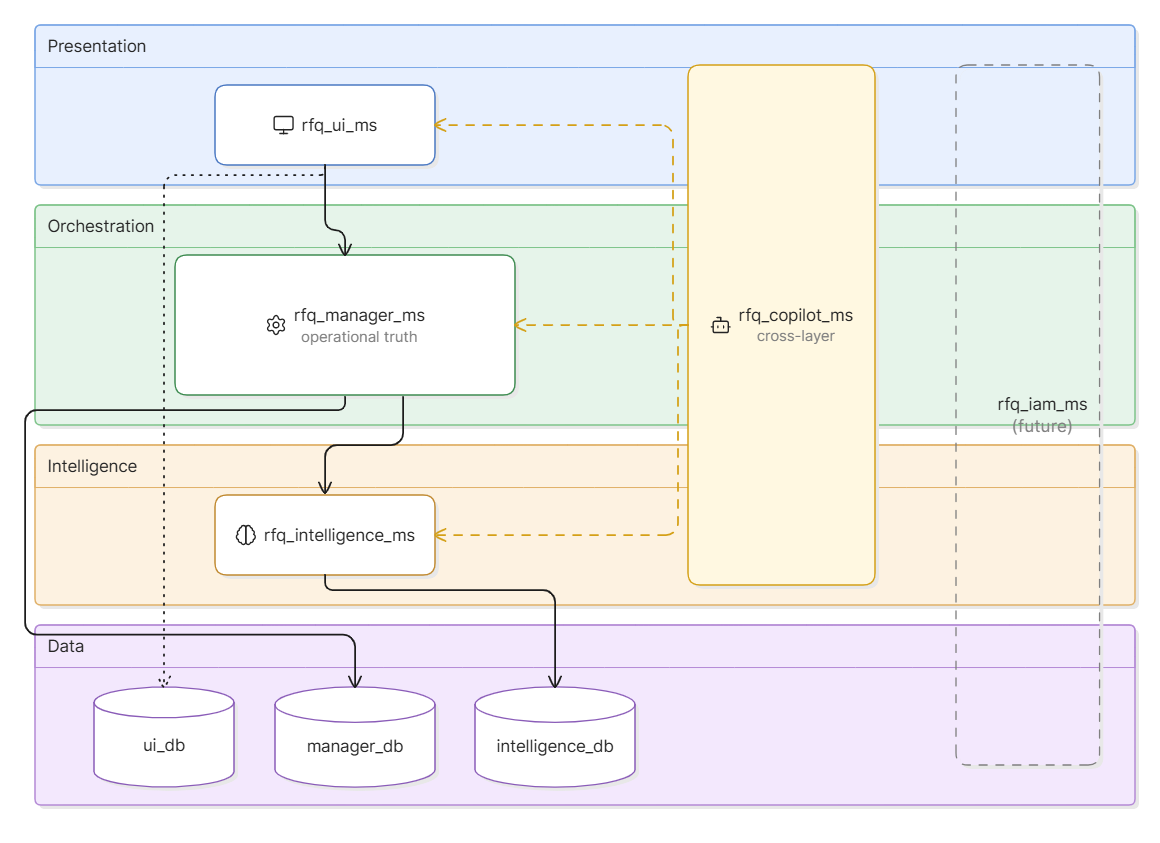
\includegraphics[width=\linewidth]{images/fig_4_1_itqan_global.png}%
        }{%
            \begin{minipage}[c][8cm][c]{14cm}
                \centering
                \textit{[Figure 4.1 placeholder: Itqan global architecture showing the four layers (presentation, orchestration, intelligence, data), the four implemented services and the future-scope IAM service, and the cross-cutting position of the RFQ Copilot as a consumer that traverses presentation, orchestration, and intelligence without owning data.]}
            \end{minipage}%
        }
    }
    \caption{Global architecture of the Itqan platform: mapping of the four layers, microservices, and the cross-cutting RFQ Copilot}
    \label{fig:itqan_global}
\end{figure}

\subsection{The Four Pillars as an Architectural Map}
The four capability pillars introduced in Chapter~\ref{chap:context} are mapped strictly to designated primary services: \textbf{Workflow and Tracking} is governed exclusively by the manager service; \textbf{Communication Automation} is partially realized via the manager service's reminder infrastructure (with outbound multi-channel delivery designated as future scope); \textbf{Business Intelligence and Executive Visibility} is co-orchestrated by the manager service (data aggregation) and the user interface (dashboarding); \textbf{Historical Learning and Predictive Analytics} is anchored in the intelligence service through deterministic document parsing, with advanced probabilistic modeling deferred. Table~\ref{tab:pillar_scope} details the operational status of each pillar.

\begin{table}[H]
\centering
\renewcommand{\arraystretch}{1.4}
\begin{tabularx}{\textwidth}{|p{3.5cm}|p{2.3cm}|>{\RaggedRight\arraybackslash}X|}
\hline
\rowcolor{lightgray}
\textbf{Pillar} & \textbf{Status} & \textbf{Architectural Coverage} \\ \hline
Workflow and Tracking & Implemented & Acts as the operational backbone of the platform, executed via the manager service across all primary lifecycle entities. \\ \hline
Communication Automation & Partial & Internal reminder infrastructure is deployed within the manager service; advanced outbound orchestration and inbound parsing remain future architectural extensions. \\ \hline
Executive Intelligence and BI & Partial & Real-time analytical endpoints are operational within the manager service; extensive BI reporting forms the future scope. \\ \hline
Historical Learning and Prediction & Foundation only & Deterministic parsing of Material Requisitions and estimation workbooks is operational within the intelligence service; predictive algorithms remain future scope. \\ \hline
\end{tabularx}
\caption{Operational scope of the four architectural pillars within the present project phase}
\label{tab:pillar_scope}
\end{table}

\section{Microservices Inventory and BACAB Pattern}\label{sec:bacab_pattern}
\subsection{Service Inventory}
The distributed platform architecture is composed of \textbf{five microservices}: four are currently operational or partially implemented, while one is architecturally deferred. \texttt{rfq\_manager\_ms} constitutes the lifecycle orchestration backbone. \texttt{rfq\_copilot\_ms} encapsulates the trust-bounded conversational layer. \texttt{rfq\_intelligence\_ms} executes deterministic data extraction over engineering documents. \texttt{rfq\_ui\_ms} serves as the presentation layer integrating live API consumption. \texttt{rfq\_iam\_ms} represents the deferred Identity and Access Management service; crucially, the manager service already embeds the requisite IAM integration point (Authorization-header forwarding and an identity-resolution connector, with token validation delegated to the future service). The microservice boundaries strictly mirror data ownership paradigms: the manager owns operational state, the intelligence service owns analytical models, the copilot encapsulates solely conversational state, and the UI owns presentation logic. This rigorous data encapsulation enables the trust-boundary architecture (Section~\ref{sec:trust_boundary}): because the copilot holds no operational truth, its outputs must invariably rely on mediated evidence from authoritative backend services.

\subsection{The BACAB Layered Pattern}
Internally, each backend service adheres to the HostCompany architectural conventions, adapted into the \textbf{BACAB layered pattern}. This structure processes requests through five \textbf{active layers}: \texttt{routes} (HTTP ingress and syntactic validation), \texttt{controllers} (domain business logic), \texttt{datasources} (persistence abstraction), \texttt{translators} (Data Transfer Object (DTO) boundary transformations), and \texttt{connectors} (external service integration, including LLM APIs). These are transversally supported by three auxiliary layers: \texttt{models}, \texttt{config}, and \texttt{utils}. Three invariant architectural principles are strictly enforced: routing layers isolate business logic; controllers abstract database operations; and data access layers execute no domain decisions. Figure~\ref{fig:bacab_pattern} illustrates this topology. The copilot service inherits this structural skeleton while injecting a specialized \texttt{pipeline} layer to orchestrate the trust-bounded LLM stages defined in Section~\ref{sec:trust_boundary}.

\begin{figure}[H]
    \centering
    \setlength{\fboxsep}{5pt}
    \setlength{\fboxrule}{0.5pt}
    \fbox{
        \IfFileExists{images/fig_4_2_bacab_pattern.png}{%
            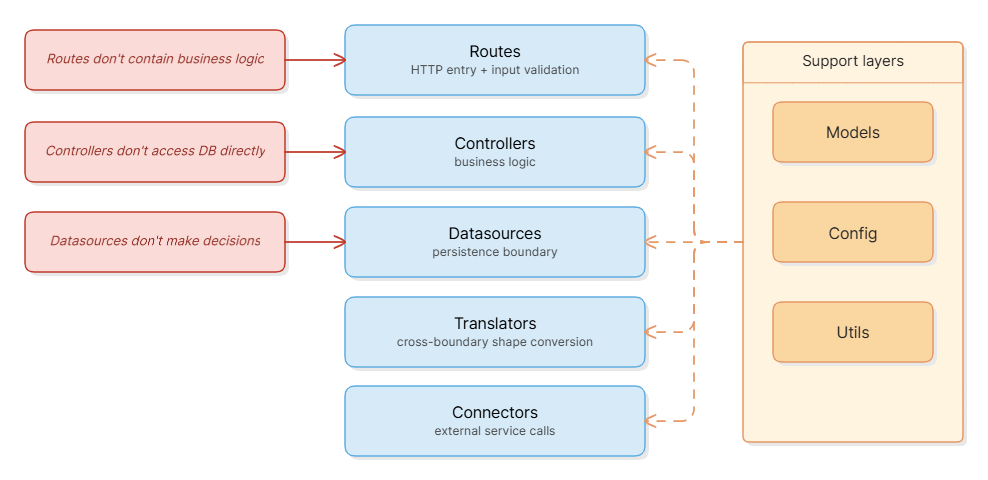
\includegraphics[width=\linewidth]{images/fig_4_2_bacab_pattern.png}%
        }{%
            \begin{minipage}[c][7cm][c]{14cm}
                \centering
                \textit{[Figure 4.2 placeholder: BACAB layered pattern. Five active layers shown vertically in request-path order (Routes $\rightarrow$ Controllers $\rightarrow$ Datasources $\rightarrow$ Translators $\rightarrow$ Connectors), three support layers (Models, Config, Utils) shown as a sidebar serving the active layers, with the three discipline rules annotated.]}
            \end{minipage}%
        }
    }
    \caption{The BACAB layered architecture: structural separation of concerns via active and supporting layers}
    \label{fig:bacab_pattern}
\end{figure}

\subsection{Inter-Service Communication}
Inter-service communication is governed by three strict protocols. \textit{Contracts:} Integration utilizes synchronous REST over HTTP, with each service exposing a versioned OpenAPI specification as the absolute source of truth. \textit{Errors:} Exception payloads follow a standardized, structured format (HTTP status, machine-readable semantic type, and human-readable context). Access violations are explicitly categorized (\texttt{401} Unauthenticated, \texttt{403} Unauthorized, \texttt{404} Resource Obfuscation for unauthorized actors). The manager service currently injects correlation identifiers, with holistic distributed tracing flagged as a hardening direction. \textit{Access Control:} The copilot is strictly prohibited from bypassing manager-mediated authorization; all evidence retrieval traverses the manager's authenticated endpoints via explicit actor-context propagation, cementing the security premise of the trust-bounded architecture.

\section{Manager Service: Domain Model and Lifecycle}\label{sec:manager_domain}
\subsection{Mission and Domain Model}
The manager service operates as the absolute operational authority within the platform: it enforces a structured, deterministic lifecycle state machine for each RFQ. Its domain scope is deliberately bounded; the execution of cost estimation remains with human experts (Chapter~\ref{chap:context}), and complex analytical synthesis is delegated to the intelligence service. The persistence schema revolves around seven core entities (Figure~\ref{fig:manager_erd}): the \textbf{RFQ} (aggregate root, encapsulating metadata and state); the \textbf{Workflow} (versioned lifecycle template); the \textbf{RFQ\_Stage} (instantiated operational node detailing transition requirements); the \textbf{Subtask} (granular execution unit supporting recursive progress aggregation); the \textbf{Note} (immutable append-only artifact); the \textbf{File} (document blob reference); and the \textbf{Reminder} (temporal automation trigger). Auxiliary mapping and configuration tables support this schema, as detailed in Chapter~\ref{chap:implementation} (Section~\ref{sec:db_schema}).

\begin{figure}[H]
    \centering
    \setlength{\fboxsep}{5pt}
    \setlength{\fboxrule}{0.5pt}
    \fbox{
        \IfFileExists{images/fig_4_3_manager_erd.png}{%
            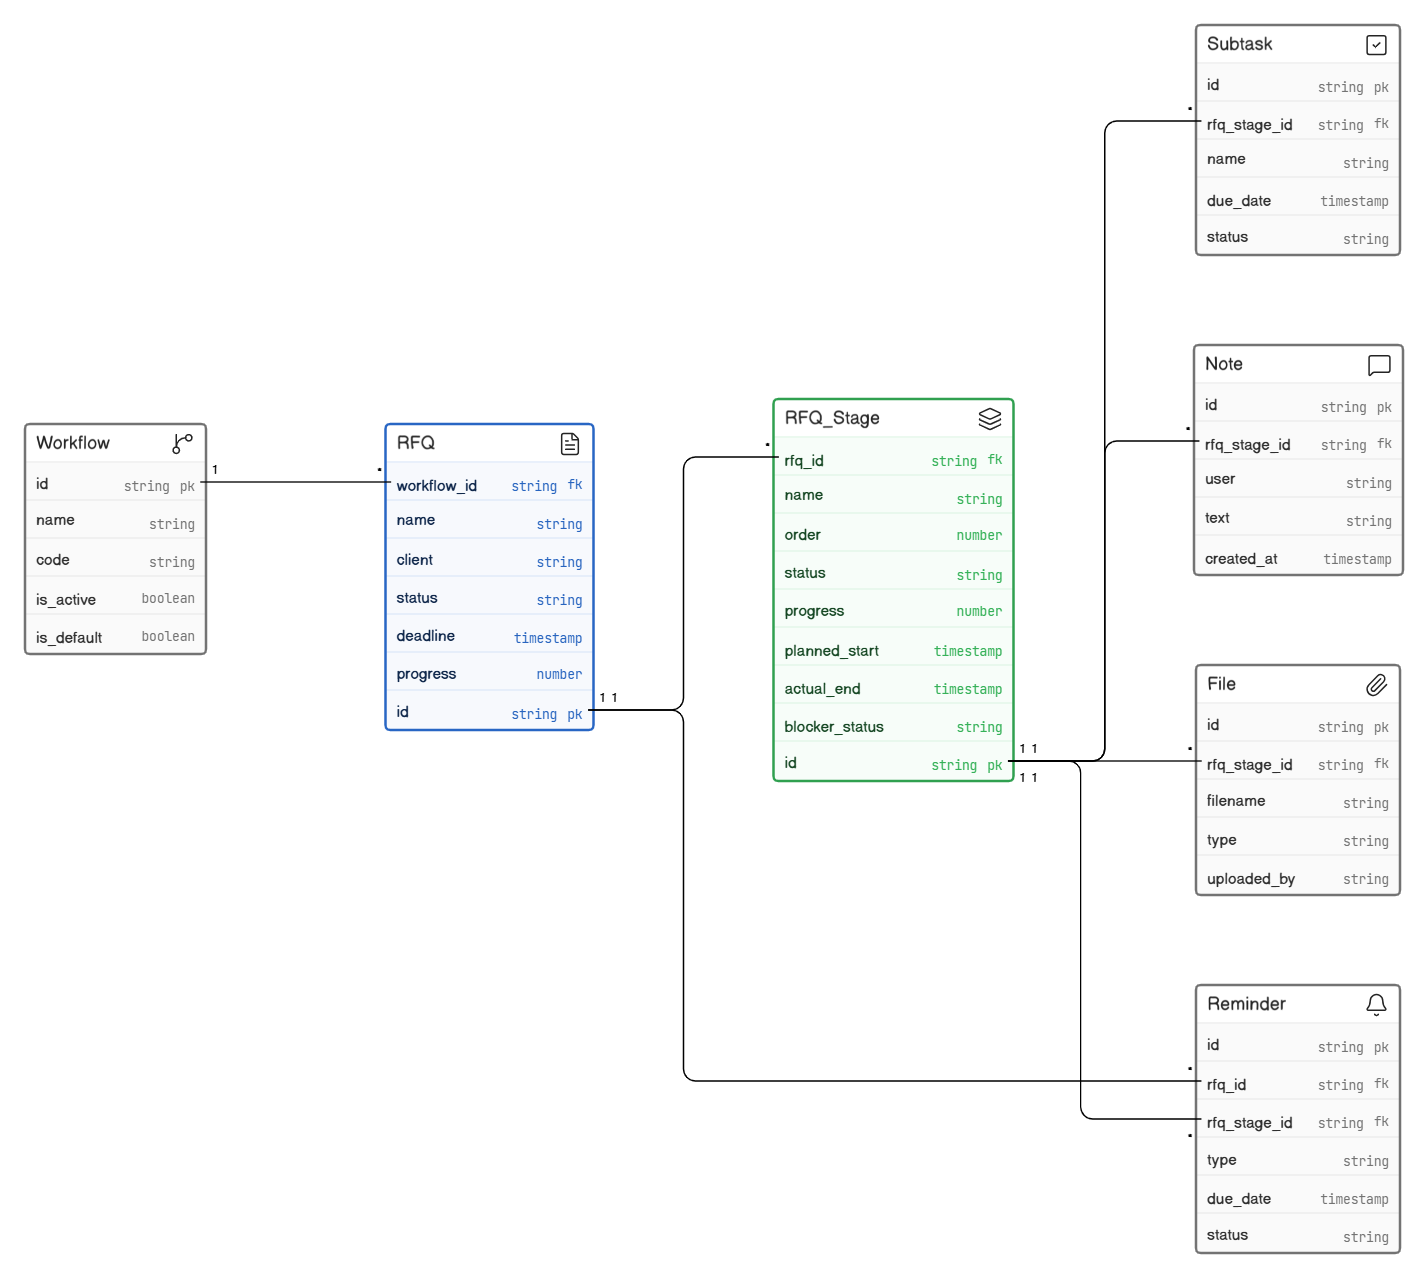
\includegraphics[width=\linewidth]{images/fig_4_3_manager_erd.png}%
        }{%
            \begin{minipage}[c][6cm][c]{14cm}
                \centering
                \textit{[Figure 4.3 placeholder: entity-relationship diagram of the manager service domain model, showing the seven primary entities (RFQ, Workflow, RFQ\_Stage, Subtask, Note, File, Reminder) and their cardinalities.]}
            \end{minipage}%
        }
    }
    \caption{Entity-relationship diagram detailing the domain model of the manager service}
    \label{fig:manager_erd}
\end{figure}

\subsection{Workflow and Stage Progression}
The structural rigidity of the manager service is enforced via its deterministic stage progression logic. The mutation of an RFQ's state across lifecycle stages represents a highly guarded transactional transition, necessitating the successful traversal of three sequential validation gates, illustrated by the \textit{Advance RFQ Stage} activity diagram (Figure~\ref{fig:activity_advance_stage}). The \textit{mandatory-field gate} aborts the transaction if predefined data dependencies for the current stage are unsatisfied. The \textit{blocker gate} halts progression if any blocking constraint, such as an unresolved feasibility or coordination issue, remains active. The \textit{transition-validity gate} enforces topological consistency, preventing arbitrary stage skipping or invalid sequencing by validating that the requested transition concerns the current active stage and follows the ordered workflow sequence. Upon the successful validation of all gates, the state mutation commits atomically: the current stage is completed with an actual end timestamp, the next pre-created stage in the workflow sequence is activated with an actual start timestamp and an in-progress status, the RFQ's current-stage pointer is updated, and progress metrics are recomputed. The technical implementation of this transactional flow resides within the controller layer and is detailed in Chapter~\ref{chap:implementation}.

\section{Copilot Service: Trust-Boundary Architecture}\label{sec:trust_boundary}
The RFQ Copilot operates explicitly as a constrained conversational interface rather than an autonomous agent. While the language model is relegated to semantic interpretation and text generation, deterministic algorithmic code strictly governs data access, tool execution, and the final authorization of responses.

This section formulates the underlying design philosophy, contrasts the copilot with alternative conversational paradigms, and defines the trust-boundary architecture that governs its pipeline logic. Implementation details are deferred to Chapter~\ref{chap:implementation}.

\subsection{Design Philosophy}
The architectural blueprint of the copilot is dictated by a singular, non-negotiable axiom:
\begin{center}
\fbox{\parbox{0.92\textwidth}{\centering\textit{The copilot must achieve conversational fluidity analogous to state-of-the-art LLMs, while explicitly abrogating their inherent generative authority. Its epistemic authority derives strictly from validated platform evidence, not from the probabilistic model.}}}
\end{center}
This axiom decisively separates \textit{fluidity} (the semantic capacity to parse intent and maintain linguistic coherence) from \textit{authority} (the factual reliability required for operational decision-making). Generic conversational systems optimize for fluidity, inadvertently projecting an illusion of authority, a catastrophic vulnerability in industrial estimation contexts, where the cost of error is asymmetric (Chapter~\ref{chap:context}). Consequently, the architecture isolates these capabilities: the language model generates fluid syntax, while deterministic microservice logic provisions and enforces absolute operational authority.

\subsection{Positioning Against Alternative Conversational AI Patterns}
The prevailing paradigms reviewed in Chapter~\ref{chap:soa} (naive RAG, autonomous LLM agents, and unconstrained function-calling architectures) exhibit a fundamental structural flaw when deployed in high-risk environments: they mistakenly grant the probabilistic language model autonomy over safety-critical decisions (e.g., context scope drift, tool selection, policy interpretation). The proposed trust-boundary architecture rectifies this by strictly reallocating responsibilities: semantic tasks (intent framing, response formulation, linguistic verification) are assigned to the LLM, whereas policy enforcement (tool authorization, evidence retrieval, logical escalation) is exclusively executed by deterministic algorithmic controls.

\subsection{The Eight Trust Boundaries}
The trust-boundary architecture isolates prompt classification from operational execution through a singular deterministic chokepoint. It systematically verifies generated responses via deterministic guardrails, culminating in a secondary LLM utilized strictly as a validating Judge. This architecture relies upon eight explicitly allocated boundaries (Table~\ref{tab:trust_boundaries}).

\newpage
\begin{table}[H]
\centering
\scriptsize
\renewcommand{\arraystretch}{1.3}
\begin{tabular}{|p{0.6cm}|p{5.5cm}|p{8cm}|}
\hline
\rowcolor{lightgray}
\textbf{\#} & \textbf{Decision Domain} & \textbf{Architectural Owner} \\ \hline
1 & Path Classification & \textit{FastIntake} (deterministic regex) or \textit{LLM Planner} (probabilistic proposal), structurally validated by the \textit{PlannerValidator} and definitively authorized by the \textit{ExecutionPlanFactory}. \\ \hline
2 & Plan Construction Authority & Exclusively the \textit{ExecutionPlanFactory}; structural uniqueness is enforced via static anti-drift syntax-tree tests in the copilot's automated test suite. \\ \hline
3 & Tool Invocation Policy & Declaratively mapped in the \textit{Path Registry} and executed exclusively by the deterministic \textit{Tool Executor}. \\ \hline
4 & Data Authorization & Controlled entirely by the manager service API; HTTP \texttt{403} or \texttt{404} responses represent absolute barriers overriding copilot intent. \\ \hline
5 & Prompt Context Boundaries & Enforced via a strict per-path field whitelist defined in the \textit{Path Registry}. \\ \hline
6 & Evidence Lineage Tracking & Per-target evidence labeling injected during the deterministic context-assembly phase. \\ \hline
7 & Output Verification & Sequential \textit{Deterministic Guardrails} followed by a terminal \textit{LLM Judge} enforcing linguistic constraint validation. \\ \hline
8 & Exception Escalation & The singular \textit{Escalation Gate}, which deterministically halts the pipeline and re-routes execution via a structured exception framework. \\ \hline
\end{tabular}
\caption{The eight deterministic trust boundaries defining the copilot's architecture}
\label{tab:trust_boundaries}
\end{table}

These boundaries are encapsulated in a unified architectural axiom: \textit{Dual classification sources, a singular execution plan factory, and a unified escalation gate. The language model exclusively generates semantics; deterministic code constructs operational truth; declarative policy enforces boundaries; the LLM Judge validates outputs; and static templates guarantee safe degradation.} Any deviation from this axiom is categorically treated as a structural violation rather than an architectural evolution. Figure~\ref{fig:canonical_pipeline} maps the canonical pipeline realizing this logic.

\begin{figure}[H]
    \centering
    \setlength{\fboxsep}{5pt}
    \setlength{\fboxrule}{0.5pt}
    \fbox{
        \IfFileExists{images/fig_4_5_canonical_pipeline.png}{%
            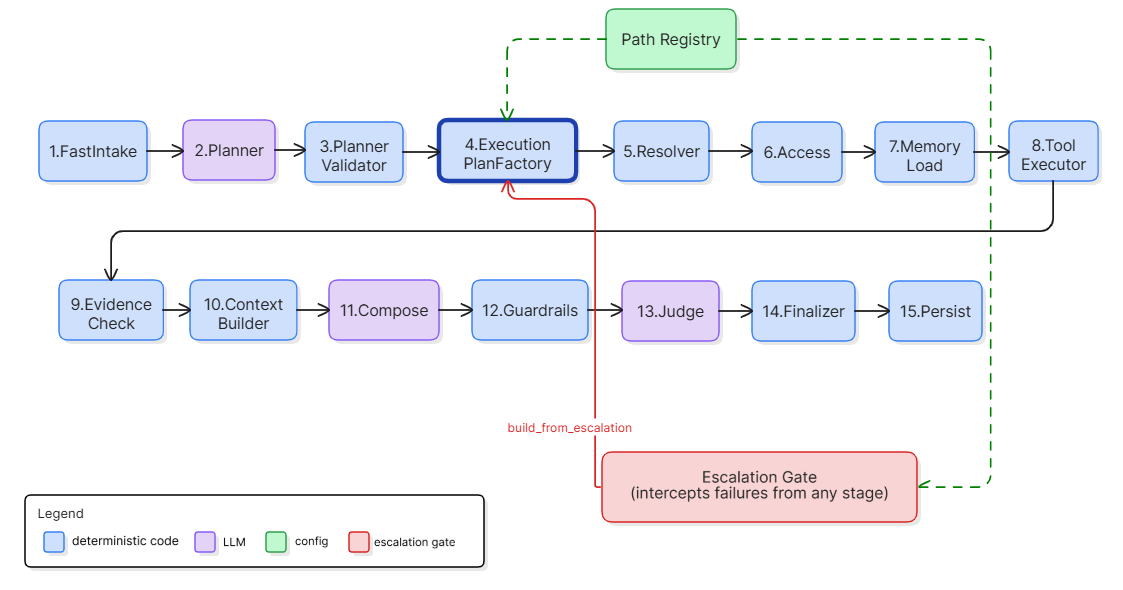
\includegraphics[width=\linewidth]{images/fig_4_5_canonical_pipeline.png}%
        }{%
            \begin{minipage}[c][9cm][c]{14cm}
                \centering
                \textit{[Figure 4.5 placeholder: canonical pipeline of the RFQ Copilot. Fifteen stages (FastIntake $\rightarrow$ Planner $\rightarrow$ PlannerValidator $\rightarrow$ ExecutionPlanFactory $\rightarrow$ Resolver $\rightarrow$ Access $\rightarrow$ Memory Load $\rightarrow$ Tool Executor $\rightarrow$ Evidence Check $\rightarrow$ Context Builder $\rightarrow$ Compose $\rightarrow$ Guardrails $\rightarrow$ Judge $\rightarrow$ Finalizer $\rightarrow$ Persist) coloured by trust class: deterministic code (blue), language model (purple, three stages), Path Registry config (indigo, dashed to Factory + Gate only), Escalation Gate intercept (red), external services (green), persistence (amber). The three LLM stages are visibly bracketed by deterministic stages on either side.]}
            \end{minipage}%
        }
    }
    \caption{Canonical processing pipeline of the RFQ Copilot, demonstrating the strict encapsulation of LLM invocations within deterministic safeguards}
    \label{fig:canonical_pipeline}
\end{figure}

\subsection{Two Classification Sources, One Plan Factory}
System interactions initiate exclusively via two distinct classification sources, both converging strictly onto a single point of execution plan construction. \textbf{FastIntake} serves as a deterministic classifier, identifying non-operational inputs (e.g., greetings, syntactic noise) utilizing anchored regular expressions, entirely bypassing the LLM. Conversely, complex intents are routed to the \textbf{LLM Planner}, which generates a probabilistic classification and data retrieval proposal. This proposal is intercepted by the \textbf{PlannerValidator}, which enforces strict schema conformance without executing policy logic. Both streams terminate at the \textbf{ExecutionPlanFactory}, the absolute single source of truth authorized to instantiate a \texttt{TurnExecutionPlan}. This singleton constraint is aggressively enforced via static anti-drift tests evaluating the project's syntax tree. Any execution anomaly triggers the Escalation Gate, forcing a deterministic fallback (Path 8) response.

\subsection{The Path Registry as Policy-as-Configuration}
The Path Registry operationalizes the \textit{policy-as-configuration} paradigm, defining the copilot's complete functional surface in a declarative matrix. It specifies permissible intake vectors, authorized retrieval tools, strict field whitelists, guardrail configurations, and targeted LLM Judge criteria for every intent path. Because policies are extracted from executable code into declarative configuration, altering systemic behavior constitutes a deterministic configuration update rather than a hazardous programmatic rewrite.

\subsection{The Pipeline and the Five Evidence Sources}
Execution traverses an immutable sequence: Intake $\rightarrow$ Factory $\rightarrow$ Resolver $\rightarrow$ Access $\rightarrow$ Memory $\rightarrow$ Tool Executor $\rightarrow$ Evidence Check $\rightarrow$ Context Builder $\rightarrow$ Compose $\rightarrow$ Guardrails $\rightarrow$ Judge $\rightarrow$ Finalize $\rightarrow$ Persist. The language model is explicitly bracketed at the Planner, Compose, and Judge nodes (Figure~\ref{fig:canonical_pipeline}). The system recognizes five epistemic evidence sources: the \textbf{conversation context} (for trivial routing), \textbf{manager service state} (primary operational truth), \textbf{intelligence artifacts} (parsed engineering data), \textbf{controlled domain knowledge} (regulatory standards), and crucially, the \textbf{absence of evidence} (enforcing explicit refusal over probabilistic approximation).

\subsection{Why This Architecture Represents the Project's Primary Innovation}
The trust-boundary architecture transcends conventional conversational prototyping through rigorous structural and operational discipline. Structurally, it isolates the probabilistic LLM from execution authority via strict type definitions and self-defending static analysis (anti-drift tests). Operationally, every critical systemic decision is delegated to highly observable, deterministically auditable components (e.g., the Path Registry, the Tool Executor, the Guardrails). Academically, this architecture provides a replicable, engineered solution to deploying LLM agents in environments where the asymmetrical cost of error precludes autonomous generative behavior.

\section{Evidence Boundary}\label{sec:pipeline_vertical_slicing}
The \textit{evidence boundary} represents the architectural invariant ensuring that the context supplied to the LLM is finite, explicitly authorized, and deterministically bounded prior to generative composition. At the \textit{path level}, the ExecutionPlanFactory leverages the Path Registry to statically enforce which systemic data sources are permitted. At the \textit{turn level}, the framework rigorously applies a per-path field whitelist and explicit evidence-lineage tagging to prevent context dilution and subsequent hallucination.

This boundary is rendered enforceable (rather than merely aspirational) via the declarative policy-as-configuration model, the singleton ExecutionPlanFactory constraint, and the sequential execution of deterministic guardrails followed by the LLM Judge. The Judge acts strictly as the terminal line of defense against semantic anomalies, never as the primary enforcer of access policy.

\section{Platform Integration and ADR Summary}\label{sec:integration}
\subsection{Platform Integration}
The platform integration model dictates that no microservice may act as the secondary persistent owner of another service's domain data. The user interface integrates live REST endpoints from the manager (lifecycle orchestration) and intelligence (deterministic extraction) services, with a demo/mock fallback retained for development, while providing contextual access to the copilot interface.

\subsection{Architectural Decisions}
Critical architectural decisions (including the adoption of microservices, the BACAB intra-service topology, the centralization of lifecycle authority within the manager service, the policy-as-configuration framework, and the trust-bounded conversational paradigm) are documented within Architectural Decision Records (ADRs). These records detail the context, alternatives considered, chosen methodologies, and resulting operational consequences, as summarized in Appendix~\ref{app:adr} (Table~\ref{tab:decisions}). The trust-boundary architecture (Section~\ref{sec:trust_boundary}) represents the most consequential structural commitment, dictating the entire behavioral profile of the intelligence layer.

\section*{CONCLUSION}
\addcontentsline{toc}{section}{CONCLUSION}
This chapter has formulated the comprehensive technical architecture of the Itqan platform: delineating the four-layer topological map, the five-service distributed framework, the intra-service BACAB pattern, and the deterministically guarded lifecycle within the manager service. Crucially, it established the trust-boundary architecture that safely encapsulates LLM capabilities within strict operational constraints, mitigating the severe risks of uncontrolled generative AI in industrial contexts. The subsequent chapter translates this conceptual architecture into precise programmatic implementation.
